\documentclass[pageno]{jpaper}

\usepackage[normalem]{ulem}
\usepackage{amsmath}

% Comment commands - easy to remove
\usepackage{color}
\definecolor{orange}{rgb}{1,0.5,0}
\newcommand{\jbs}[1]{{\color{blue}[\textbf{\sc JBS}: \textit{#1}]}} %Josef
\newcommand{\dhp}[1]{{\color{red}[\textbf{\sc DHP}: \textit{#1}]}} %Dong-hyeon
\newcommand{\ab}[1]{{\color{magenta}[\textbf{\sc AB}: \textit{#1}]}}%Akhil
\newcommand{\fh}[1]{{\color{orange}[\textbf{\sc FH}: \textit{#1}]}}  %Fabiha
\newcommand{\es}[1]{{\color{Green}[\textbf{\sc ES}: \textit{#1}]}}  %Eric

\begin{document}

\title{Sphynx: A Shared Instruction Cache Exporatory Study}

\author{Dong-hyeon Park \and Akhil Bagaria \and Fabiha Hannan \and
  Eric Storm \and Josef Spjut}

\date{}
\maketitle

\thispagestyle{empty}

\begin{abstract}
The Sphynx project was an exploratory study to discover what might be
done to improve the heavy replication of instructions in independent
instruction caches for a massively parallel machine where a single
program is executing across all of the cores. 
It is expected that a large amount of sharing should be possible when
the independent threads all issue from the same instruction pool.
Ideally a large amount of sharing should be possible, where a single
instruction cache can be shared among $N$ threads, where $N\geq 2$.

\end{abstract}

\section{Introduction}

\jbs{I expect this entire paper to be about 3-4 pages. We should be clear
and concise, but still put all our ideas down.}

Instruction caches are widely used to mediate the effects of reads from main memory, relative to computation time. 
The instruction cache is accessed for every instruction executed and program execution time can vary widely depending on the number of instruction cache misses~\cite{arnold94}. 
In existing Graphics Processing Units (GPUs) and CPUs, each processor core has its own instruction cache. 
A unified or shared instruction cache that is used by all, or many cores of a GPU or CPU has the potential to improve system performance and reduce power consumption.
However, such a modification also results in increased traffic for the instruction cache, which could lead to a higher miss rate, reducing performance and increasing power consumption. 
In current computer architectures, the instruction caches are independent of one another, however since each processor uses the same set of instructions, it is plausible that a shared instruction cache could introduce non-trivial improvements in performance. 
Unified instruction cache(s) could reduce the number of compulsory misses because an instruction previously executed by one streaming multiprocessor may be available for another streaming multiprocessor immediately rather than requiring an additional miss. 
In addition to a fully unified instruction cache used across all processor cores, another possible solution could be to maintain multiple instruction caches, which are shared across a subset of all cores. 
This architecture could allow the operating system to group together program threads based on similarity of instructions to maximize the benefit of shared instructions and minimized the conflicts across threads. 

GPGPU-Sim~\cite{bakhodayuan09} is an open-source software package available to simulate GPU architecture. 
It has been validated to be representative of performance on NVIDIA GPUs and provides a reasonable platform for testing alternate highly-parallel computer architectures.
\jbs{This discussion seems more fitted to the methodology part of the results section.}

\section{Background}

Background goes here.



\section{Shared Instruction Cache Design}

Describe the instruction cache design(s) we propose testing.


\section{Results}

% expected results
There are two methods for analyzing the potential gains from shared
instruction caches.
The first is to keep the total instruction cache size across the chip
constant and increase the capacity each thread sees by grouping that
storage together.
This method of sharing will provide no area savings, but should grant
an increased hit rate for the now larger cache.
The increase will be limited by the working set of the application.
We expect that the hit rate improvement will only be minor and
therefore do not generate any results for this method.
%% We project improvement in cache performance for this approach in
%% Figure~\ref{HitImprov}. 

% \begin{figure}[b]
% \centering
% 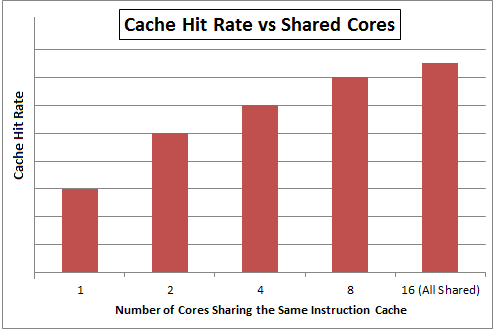
\includegraphics[width=\columnwidth]{graphics/HitRateImprov.png}
% \caption{Projected instruction cache hit rate with fixed total cache size and increased sharing}
% \label{HitImprov}
% \end{figure}

The second method is to reduce the total storage required for
instruction cache data arrays while allowing at most a minor
degredation in hit rate.
We consider an approach where the instruction cache each processor
sees remains fixed but the number of threads sharing each cache is
increased. 
We expect that the miss rate of the cache will increase when the instruction
cache is not large enough to satisfy the demands from all the cores
sharing the cache.
However, the performance penalty should not be as dramatic as the
reduction in area when all threads run the same application.
Figure \ref{AreaEff} shows our rough expectations for this approach
which should improve the efficiency of the chip.

\begin{figure}
\centering
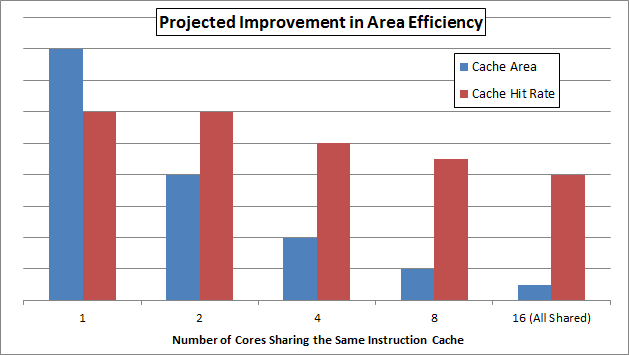
\includegraphics[width=\columnwidth]{graphics/AreaEff.png}
\caption{Projected cache area and miss rate due to increased sharing}
\label{AreaEff}
\end{figure}


\subsection{Setup}

We use GPGPU-Sim to analyze the effectiveness of our design because of
its ability to simulate a large number of parallel processing cores.
GPGPU-Sim~\cite{bakhodayuan09} is an open-source software package
available to simulate GPU architecture. 
It has been validated to be representative of performance on NVIDIA
GPUs and provides a reasonable platform for testing alternate
highly-parallel computer architectures, and provides a reference
configuration for a NVIDIA GTX580 GPU, which we used for our study.
The GTX580 contains 16 streaming multiprocessors with the NVIDIA Fermi
architecture. 
In GPGPU-Sim, each CUDA streaming multiprocessor is represented as a
single SIMT core, with all the SIMT cores placed within a single SIMT cluster. 
Each streaming multiprocressor can have up to 48 warps, with 32
threads per warp (See Table \ref{table:gpuconfig}). 
All sixteen SIMT cores share unified 786KB L2 cache. 

% \begin{figure}[b]
% \centering
% 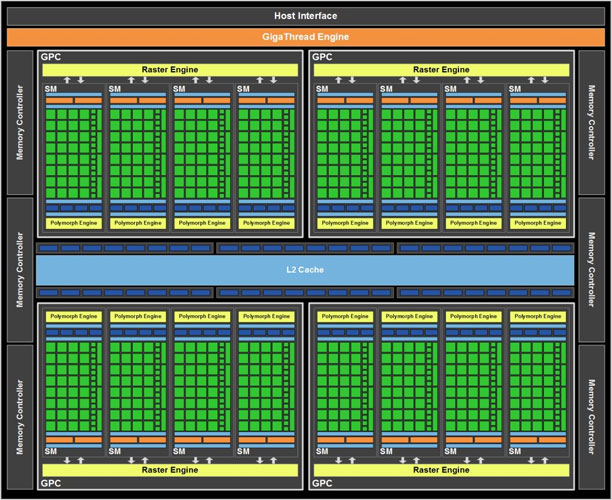
\includegraphics[width=\columnwidth]{graphics/GTX580.jpg}
% \caption{Block Diagram of NVIDIA GTX580~\cite{gf100}}
% \label{GTX580}
% \end{figure}

\begin{table}[ht]
\caption{GTX580 Configuration in GPGPU-Sim}
\begin{tabular}{l|c}
\hline\hline
SIMT cluster count & 1 \textbf{/} 2 \textbf{/} 4 \textbf{/} 8 \textbf{/} 16  \\
\hline
Cores per cluster & 1 \\
\hline
Memory controller count & 6 \\
\hline
Subpartition per mem. & 2 \\ 
\hline
Shader registers & 32768*(16 \textbf{/} 8 \textbf{/} 4 \textbf{/} 2 \textbf{/} 1 ) \\
\hline
Threads in pipeline & 1536*(16 \textbf{/} 8 \textbf{/} 4 \textbf{/} 2 \textbf{/} 1 ) \\
\hline
Threads per warp & 32 \\
\hline
Scheduler per core & 2*(16 \textbf{/} 8 \textbf{/} 4 \textbf{/} 2 \textbf{/} 1 )\\
\hline
CTA per core & 8*(16 \textbf{/} 8 \textbf{/} 4 \textbf{/} 2 \textbf{/} 1 )\\
\hline
Core clock & 700 MHz\\
\hline
L2 \& Interconnect clock & 700 MHz\\
\hline
DRAM clock & 924 MHz\\
\hline
Topology & 13 \textbf{/} 14 \textbf{/} 16 \textbf{/} 20 \textbf{/} 28 \\
\hline
L1 Instruction Cache & 4 sets : 128B blocks : 4-way \\
\bottomrule[1pt]
\end{tabular}
\caption*{\textmd{GPGPU-Sim configurations used in simulation. Any parameter not listed in the table was kept the same from the original GTX480 configuration that is included in the GPGPU-Sim source code.}}
\label{table:gpuconfig}
\end{table}

In the Fermi architecture, each streaming multiprocessor has
its own distinct L1 cache. 
Each L1 instruction cache is 4-way set associative, with 4 sets of
128 bytes per block. 
To assess the  performance of different L1 instruction cache
architectures, only the L1 instruction cache was modified, while all
other architectural variables remained constant. 
Other aspects of the architecture such as the bandwidth of shared L2
cache could serve as a performance bottleneck for different cache
designs. 
However, these variables are ignored for this study, because we expect
them to have little impact on the hit and stall rate of the
instruction cache, which are the primary metrics of interest.

\subsection{Preliminary Results}

We used benchmarks provided by the standard GPGPU-Sim distribution
to validate our second method for sharing instruction caches by
keeping the cache the same but increasing the number of threads that
share that cache.
This means varying the number of SMs per instruction cache from 1 to
16 (the maximum number of cores available on the GTX580).
Note that since each SM can have up to 48 warps, the number of
simultaneously executing threads sharing the same instruction cache is
much larger than the SM count.
The results can be seen in Figures~\ref{fig:missStalls}
and~\ref{fig:missStallsZoomed}. 
As expected, the miss rate increases slightly in most cases by the
increased pressure on the shared cache.
A couple benchmarks were more problematic and resulted in up to nearly
a 45\% stall rate when shared by 16 threads.
We provide observations about those benchmarks in
Section~\ref{sec:benchmarks}.

\begin{figure}
\centering
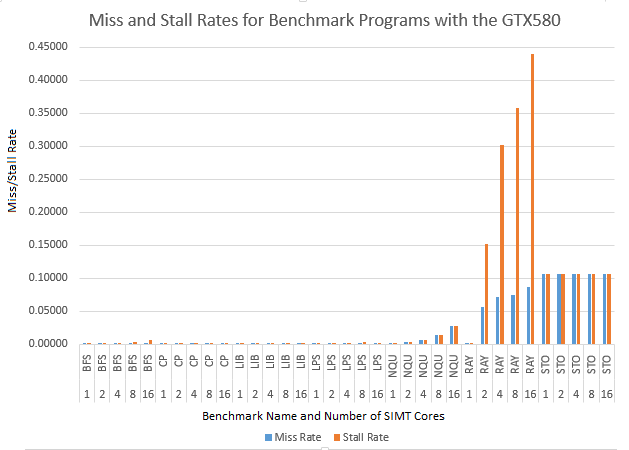
\includegraphics[width=\columnwidth]{graphics/miss_stalls_benchmarks.png}
\caption{Simulated Miss and Stall Rates}
\label{fig:missStalls}
\end{figure}

\begin{figure}
\centering
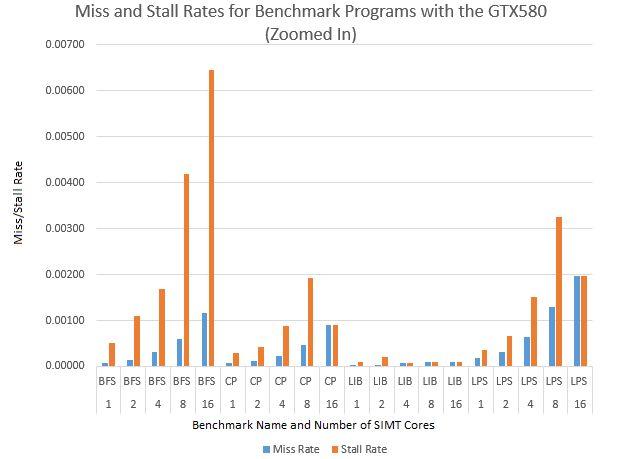
\includegraphics[width=\columnwidth]{graphics/miss_stalls_benchmarks_zoomed.png}
\caption{Simulated miss and stall rates (zoomed in) }
\label{fig:missStallsZoomed}
\end{figure}

For the cases where the miss rate become unacceptable under increased
sharing, we should instead allow for the cache to also increase in
capacity. 
However, capacity alone will only affect the miss rate reported from
the simulations.
The stall rate represents the percentage of cache accesses that fail
due to the increased pressure on the cache from sharing without
increasing the available read parallelism.
We expect that simply allowing for independent banks of the
instruction cache to be accessed independently would overcome this
limitation, but we have not yet simulated this approach.
However, other high-level simulation has shown this kind of
instruction cache banking scheme to be potentially
effective~\cite{kopta10}. 

% can we include results for the increased cache size tests?

%% The performed simulations point to several factors that may account 
%% for the outcomes seen with each approach. Parameters that are expected 
%% to affect instruction cache performance include the number of cores 
%% shared, associativity, parallelism, and cache size.

%% The first method, varying the number of cores sharing a cache while 
%% keeping the total cache size constant, was expected to improve the hit 
%% rate. As the number of cores sharing the cache increased, the miss rate 
%% and stall rate both increased, with the later increasing more rapidly 
%% due to the higher number of reservation fails. While the hit rate may 
%% have improved, there was an overall trend of increased reservation fails 
%% because the cache was preoccupied with instructions from the greater 
%% number of cores. As an exception to this, CP demonstrated a balance as 
%% the stall rate decreased going from 8 cores to 16 cores sharing the 
%% cache. This was most likely due to the higher level of parallelism that 
%% CP had in comparison to the other benchmarks. Meanwhile, smaller programs 
%% remained unaffected more often than larger benchmarks.

%% The second approach entailed reducing the total cache size by keeping 
%% the size of each individual instruction cache constant when merging the 
%% cores that share each one. The reduction in area of the now shared cache 
%% allowed duplicate instructions to be accessed more quickly. This 
%% affected benchmarks with many reused instructions and is expected to 
%% provide space to be used for other caches.

%% Overall, these methods appear to perform best on multi-threaded 
%% applications with many reused instructions. Meanwhile, for benchmarks 
%% with higher hit rates to begin with, and thus less reservation fails, 
%% this method made less of an impact.

\subsection{Benchmarks}
\label{sec:benchmarks}
The result of varying the number of SM sharing from 1 to 16 is shown in Figure~\ref{fig:missStalls}, and Figure~\ref{fig:missStallsZoomed} shows 
a zoomed in version of the same data. A total of seven benchmarks were
tested, and they all came with the GPGPU-Sim source code \cite{bakhodayuan09}.

The benchmark STO is mostly unaffected by the increase in number of cores
accessing the same small instruction cache, and the benchmark shows similar
level of miss and stall rate. 
On the other hand, RAY exhibits a much higher stall rate than its miss rates in Figure~\ref{fig:missStalls}, 
and is evidently more sensative to increased sharing of the cache.
Higher stall rate compared to miss rate occurs when the cache is not able to 
respond to the CPU on time, even when there is a cache hit.
The rapid increase in stall rate in RAY and the relatively modest increase in miss rate 
suggests the cache is not able to handle the rapid increase in the amount of requests coming from the cores,
and has to stall even when there is a hit.

As RAY showed to have the largest number of PTX instructions amongst our set of benchmarks,
the high miss and stall rate is reflective of the high level of instruction cache utilization
by the benchmark. 

Similar relationship between stall rate and miss rate are also evident in 
benchmarks BFS, CP, and LPS. However, the miss rate of less than 1\% in these benchmarks
suggests that the benchmarks are largely affected by initial compulsary misses, and operate
largely on a small set of instructions.

% \emph{CP (Coulombic Potential)}

% Given a standard configuration, CP issues a high number of thread
% blocks -- a representation of the high degree of parallelism that CP
% utilizes.

% \emph{Ray (Ray Tracer)}

% RAY was the most interesting bechmark because it had the highest
% number of PTX instructions issued and was also significatly parallel. 
% Moreover, the fact that the degree of parallelism of RAY could be
% increased easily by modifying the parameters to the CUDA program.
% By increasing the size of the picture to 512 by 512, we made RAY issue
% a much higher number of thread blocks per unit time. 
% This ensured that the RAY benchmark was executing as parallel in
% software as the Coulombic Potential benchmark in the number of work
% elements that it was issuing. 
% Given that the RAY CUDA file issues more instructions in its core
% computation that CP does, and that a lot of its instructions (CUDA
% instructions) seem to be computationally more expensive, RAY can now
% be treated as both a long program which would occupy a significant
% amount of space in the instruction cache (and hence would not be
% entirely resident in the instruction cache) AND would issue those
% instructions with a high degree of parallelism.

\section{Conclusions}

\jbs{Dong-hyeon in charge}

Describe the take away from our proposed work direction.

Future work.

Other thoughts?



\section*{Acknowledgement}
We acknowledge that this idea for reducing the instruction cache area
overhead by aggressively sharing the cache originally came from
previous work on the TRaX
architecture~\cite{spjut08,spjut09,kopta10,spjut12,kopta13,kopta14}.
The TRaX architecture was designed for ray tracing and supports
thousands of threads running the same application but working on
different data.

\bstctlcite{bstctl:etal, bstctl:nodash, bstctl:simpurl}
\bibliographystyle{IEEEtranS}
\bibliography{references}


\end{document}

